\section{Introduction - Computational Models for Condensed Matter Physics}
\label{chap:Introduction}

Condensed matter physics is a branch of physics exploring microscopic and macroscopic behaviors of systems comprised of "atomic units" with interatomic interactions.  Without interactions between particles, all matter would behave like an ideal gas; interactions are what produce the rich variety of material behaviors we observe.  Because of interatomic interactions, gases can condense into liquid and solid phases and exhibit far greater complexity.  Condensed matter physics models these emergent phases of matter to address questions in material science inquiries, biological matter, and fundamental physics.  Its mathematical and theoretical framework draw upon the laws of thermodynamics, the statistical behavior of macroscopic systems, the underlying quantum mechanics of all matter, and the language of field theories, some of which will be explored in more detail herein.

Beyond the mechanics of ordinary liquids and solids, condensed matter physics encompasses the study of superconductivity, magnetism, quantum phase transitions, electronic band structure, continuum models of elasticity, and more.  Apparent differences between these phenomena often hide deep universalities that arise from underlying symmetries and that have important implications for both theory and application.

Early studies of condensed matter physics were primarily concerned with the macroscopic behaviors of common materials subject to changes in their environment.  The effects of heating, cooling, and doing work on a system, mechanical or otherwise, gave rise to the laws of thermodynamics and the description of engines.  Familiar names like Joules and Kelvin adorn many of the relationships and units of measure of thermodynamic variables.  Despite its basis in experiment and direct observation, important yet invisible descriptions of the energetics of these systems in terms of entropy and thermodynamic potentials became apparent.

A crowning achievement of the late 19th century was the development of a statistical framework that established relationships between the classical mechanical description of interactions among particles and the thermodynamic description of matter, particularly as the number of these particles becomes large.  Despite tremendous success in marrying macroscopic behavior with the coordinated actions of individual particles interacting through known forces, anomalies were known, particularly at low temperatures close to absolute zero.  As the quantum nature of matter began to be revealed, quantum statistical mechanics provided convincing answers to these anomalies and gave physicists the tools to understand macroscopic systems under a wide range of physical states and environmental conditions.

In the first pages of many a textbook about statistical mechanics, the description of a system of $N$ interacting particles introduces the idea of a microstate $\mu_M$, or a complete description of the state of the system in terms of $6N$ coordinates in $3D$ position and momentum space.  Given such a description and an appropriate Hamiltonian $\mathcal{H}(\mu_M)$ for the energy of a particular microstate, the time evolution $\mu_M(t)$ follows Hamiltonian mechanics and in principle allows for "perfect knowledge" of the behavior of the system.  Practically speaking, given any more than just a few particles, this $6N$-dimensional phase space can only be solved numerically and leads quite naturally to a branch of condensed matter physics known as molecular dynamics (MD) simulations.  The computational limits of such a model, both in terms of large $N$ and long timescales, gives rise to a variety of important approximations and new models.

\subsection{Molecular dynamics description}

A molecular dynamics (MD) description of a system is one of several models that aims to interrogate the behavior of "atoms", or particles, in a condensed matter system.  Although the term "atom" can be taken literally to mean any element from the periodic table, refinements of MD simulations often will deal with "particles" which represent clusters of atoms, molecules, or even larger units.  At their core, MD simulations do exactly what was described above.  Namely, they begin with a microstate (a point in $6N$-dimensional phase-space) together with an appropriate Hamiltonian, and time-evolve a system according to the laws of Newtonian mechanics.  The method of MD simulations can then be applied to a wide variety of material systems, including liquids and crystalline solids in two and three dimensions, plasmas, and biological structures, to name but a few.

\begin{figure}[!htbp]
  \centering
  \begin{tikzpicture}[
    atom/.style={circle, draw, fill=gray!50, minimum size=8pt, inner sep=0pt},
    bond/.style={line width=0.8pt},
    angle arc/.style={draw, line width=0.5pt},
    psi arc/.style={draw, Stealth->, line width=0.5pt},
    label/.style={font=\small, anchor=south},
    every node/.style={font=\small}
  ]
  
  % Layout positions
  \coordinate (A1) at (0,3);   % Bonds
  \coordinate (A2) at (6,3);   % Simple Angles
  \coordinate (B1) at (0,0);   % Dihedral φ
  \coordinate (B2) at (6,0);   % Dihedral ψ
  
  % === Bonds ===
  \node[atom] (b1) at ($(A1)+(-0.5,0)$) {};
  \node[atom] (b2) at ($(A1)+(0.5,0)$) {};
  \draw[bond] (b1) -- (b2);
  \node[label] at ($(A1)+(0,-0.5)$) {$r$};
  \node[font=\bfseries] at ($(A1)+(0,1)$) {Bonds: $U(r)$};
  
  % === Simple Angles ===
  \node[atom] (a1) at ($(A2)+(0,0.5)$) {};
  \node[atom] (a2) at ($(A2)+(-1.0,-0.25)$) {};
  \node[atom] (a3) at ($(A2)+(1.0,-0.25)$) {};
  \draw[bond] (a1) -- (a2);
  \draw[bond] (a1) -- (a3);
  \draw[angle arc] ($(A2)+(-0.325,+0.2)$) arc[start angle=210,end angle=330,radius=0.4];
  \node at ($(A2)+(0,-0.3)$) {$\theta$};
  \node[font=\bfseries] at ($(A2)+(0,1)$) {Simple Angles: $U(\theta)$};
  
  % === Dihedral: $U(\phi)$ ===
  \node[atom] (d1) at ($(B1)+(-0.8,0.2)$) {};
  \node[atom] (d2) at ($(B1)+(-0.4,-0.5)$) {};
  \node[atom] (d3) at ($(B1)+(0.4,-0.3)$) {};
  \node[atom] (d4) at ($(B1)+(0.6,0.3)$) {};
  \draw[bond] (d1) -- (d2) -- (d3) -- (d1);
  \draw[bond] (d2) -- (d3) -- (d4) -- (d2);
  \draw[dashed] (d1) -- ($(d2)!0.5!(d3)$) -- (d4);
  \draw[angle arc] ($(d2)!0.5!(d3)+(0.2,0.275)$) arc[start angle=40,end angle=130,radius=0.4];
  \node at ($(d2)!0.5!(d3)+(0.0,0.7)$) {$\phi$};
  \node[font=\bfseries] at ($(B1)+(0,1)$) {Dihedral Angles: $U(\phi)$};
  
  % === Improper: $U(\psi)$ ===
  \node[atom] (p1) at ($(B2)+(-1.0,0.3)$) {};
  \node[atom] (p2) at ($(B2)+(-0.8,-0.4)$) {};
  \node[atom] (p3) at ($(B2)+(0.4,-0.2)$) {};
  \node[atom] (p4) at ($(B2)+(0.6,-0.9)$) {};
  \draw[bond] (p1) -- (p2) -- (p3) -- (p4);
  \draw[->, line width=0.5pt] ($(p2)!0.5!(p3)+(0.2,-0.3)$) arc[start angle=290,end angle=110,radius=0.3];
  \node at ($(p2)!0.5!(p3)+(0.2,0.4)$) {$\psi$};
  \node[font=\bfseries] at ($(B2)+(0,1)$) {Improper Angles: $U(\psi)$};
  
  \end{tikzpicture}
  \caption{Common bond potentials in an MD simulation.}
  \label{fig:md-potentials}
\end{figure}

A typical MD calculation begins by initializing a system with a set of molecules in a simulation box, with predetermined intramolecular bonds between the atoms.  Atoms are assigned positions and momenta at locations within the box and with momenta sampled from the temperature-dependent Maxwell-Boltzmann distribution.  The system's energy is given by evaluating the kinetic energy of the atoms and the evaluation of potential energy, commonly broken down by electrostatics, bond lengths, and angles between bonds, as depicted in Fig.~\ref{fig:md-potentials}.  The MD description of a system has strong analogies to a spring-block system with a variety of blocks of differing masses representing different types of atoms, and varieties of springs that capture the details of the aforementioned potentials, as depicted for a $2D$ system in Fig.~\ref{fig:spring_mass_grid}.  The edges of the simulation box itself are typically treated as periodic boundaries, such that the system is effectively infinite in scope.  The trajectories of each particle are calculated according to standard Newtonian dynamics as calculated from the various potentials described above, with new position and momentum vectors updated appropriately for each atom after every time step.  These trajectories are then analyzed, usually by calculating a variety of statistics, to answer an investigator's particular inquiries into the behavior of the system.

\begin{figure}[!htbp]
  \centering
  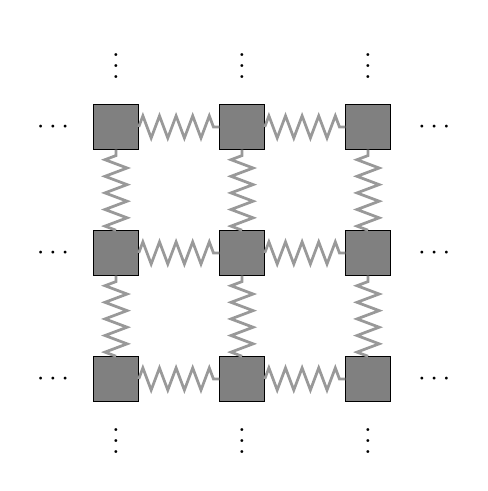
\begin{tikzpicture}[scale=1.6, 
    mass/.style={draw, fill=black!50, minimum size=16pt, inner sep=0pt, rectangle},
    spring/.style={decorate, decoration={zigzag, segment length=6pt, amplitude=4pt}, draw=black!40, line width=1pt}]
  
    % Define grid size
    \def\rows{3}
    \def\cols{3}
  
    % Draw masses
    \foreach \i in {0,...,2} {
      \foreach \j in {0,...,2} {
        \node[mass] (m\i\j) at (\i,\j) {};
      }
    }
  
    % Draw springs (horizontal)
    \foreach \j in {0,...,2} {
      \foreach \i in {0,1} {
        \draw[spring] (m\i\j) -- (m\the\numexpr\i+1\relax\j);
      }
    }
  
    % Draw springs (vertical)
    \foreach \i in {0,...,2} {
      \foreach \j in {0,1} {
        \draw[spring] (m\i\j) -- (m\i\the\numexpr\j+1\relax);
      }
    }
  
    % Add math-style ellipses to indicate infinite extension
    \foreach \j in {0,...,2} {
      \node at (-0.5,\j) {$\cdots$};
      \node at (2.525,\j) {$\cdots$};
    }
    \foreach \i in {0,...,2} {
      \node at (\i,-0.425) {$\vdots$};
      \node at (\i,2.55) {$\vdots$};
    }
  \end{tikzpicture}
  \caption{Representation of an infinite spring-mass lattice illustrating the essential behavior of an MD simulation.}
  \label{fig:spring_mass_grid}
\end{figure}

While the fidelity of MD simulations can be quite accurate for a wide variety of target systems, the approach has some inherent limitations.  Firstly, due in part to long-range interactions vis-à-vis the Coulomb potential, computational complexity generally scales with $N^2$, often limiting the total size of the system to thousands of atoms.  More critical, however, are the constraints on the size of individual time-steps due to the relatively rapid motion of atoms, especially at temperatures $T \gg 0$K.  For all atom simulations, $\delta t \sim 1$ femtosecond is typical, with total trajectories of $\sim 10-100$ nanoseconds can take hours or days of compute time.

A number of refinements on the MD model make it possible to push through these limits.  For example, biological systems will often employ complex water models to reproduce the behavior of the surrounding media, rather than modeling individual water molecules.  The general terminology for this approach is called "coarse-graining" and can be applied by representing groups of atoms as the "atoms" with appropriate potentials as depicted in Fig.~\ref{fig:md-potentials} for the desired groupings.  Coupled with this approach is the difficult task of defining and refining these potentials, which, even for all-atom simulations, represents an entire subfield of MD modeling.  Another significant limitation of MD simulations is that they typically don't permit chemistry to occur; that is, the bonds with which the system is initialized are permanent, and no new bonds form.

The development of new computational models for condensed matter systems was, in part, motivated by the limitations of MD simulations.  New continuum models to describe the behavior of macroscopic systems replaced a $6N$-dimensional vector space that specified the exact position and momentum of each particle with a $d$-dimensional number density field that described the probability of finding a particle at a position within the field.  These density field models have sought answers to questions ranging from the structure of valence electrons and predictions about the lowest energy configuration of atoms within a molecule or crystal, to the structure of defects within a crystallite, grain boundaries between crystallites, the nature of elastic and plastic deformations, and many more.

\subsection{Classical Density Functional Theory}
The history of density function theory (DFT) and dynamic density function theory (DDFT) can be traced back to early studies of Brownian motion by Brown, Einstein, and other giants of the late 19th and early 20th century, including Langevin, Fokker, and Planck \cite{te2020classical}.  In 1894, J. D. van der Waals investigated the liquid-gas interface, which is considered the first application of density functionals \cite{te2020classical}.  As the study of statistical mechanics progressed, especially with the work done by Gibbs on ensembles, DFT was extended to describe finite-temperature effects.

DFT can be applied to a variety of systems \cite{jaric1988density, jones1985density}, resulting in various formulations with respect to the definition of the density field, the functional form of a thermodynamic potential, and, in the case of DDFT, the formulation of an appropriate equation of motion.  Considerations include whether fields are studied in isolation, as in a single-species atomic liquid or solid, or as coupled fields, as appropriate for binaries, vector order parameters (e.g., magnetic moment, nematic ordering), and whether or not a particular field is conserved, as is the case for physical densities in a closed system, but not, for example in the case of magnetization.

For an atomic system, two key transformations are needed to convert an MD-like description of a system into a density field description.  First, instead of treating particles as a collection of discrete points $\{\vec{q}_i\}$ with instantaneous momenta $\{\vec{p}_i \}$, the short time scale motion of the atoms $\mu_M(t)$ is integrated out and converted into a field called the number density $\rho(\pos)$ around each particle's position, i.e.

\begin{align}\label{eqn:md-to-field}
\mu_M(\{\vec{q}_i, \vec{p}_i \}) \rightarrow \rho(\pos).
\end{align}
%

This concept is depicted in Fig.~\ref{fig:md-pfc-representations-timescales} with an MD-like representation of individual particles at $\vec{q}_1(t)$ and $\vec{q}_2(t)$ tracing motions within their respective potential wells shown on the left over a time scale indicated by $\tau_\mu$.  At this time scale, the $\langle \vec{q}_i \rangle$ is the equilibrium position of the $i$th atom over approximately a Gaussian distribution.  This distribution is represented on the right of the figure as a number density field $\rho(\pos)$.  Over longer time scales $\tau_D$, the equilibrium position of atoms may diffuse to a new position due to changes in external fields or long range interactions between particles.

\begin{figure}[!htbp]
    \centering
    \includegraphics[width=0.75\linewidth]{fig/fig-md-field-theory.pdf}
    \caption{Molecular Dynamics (MD) vs Field Theory Description.  MD simulations, as illustrated on the left, treat atoms as point particles in a $6N$ vector space with position and momentum vectors $(\{\mathbf{q}_i\},\{\mathbf{p}_i\})$, $i = 1, 2, \ldots, N$.  The trajectories of atoms in an MD simulation are calculated by time-stepping Newtonian equations of motion [i.e. $\mathbf{q}_i(t + \Delta t) = \mathbf{q}_i(t) + \mathbf{p}_i/m \cdot \Delta t$ and $\mathbf{p}_i(t + \Delta t) = \mathbf{p}_i(t) - \nabla U \cdot \Delta t$], with typical microscopic timescales on the order of $\tau_{\mu} = 10^{-12}$ s, making it impractical for observing diffusion.  Field theories, as illustrated on the right, integrate out the microscopic motion of the atoms to arrive at a number density field $\rho$, discretized over a regular lattice.  The change in the density field is given by $\rho(t + \Delta t) = \rho(t) + D \nabla^2 [\delta F / \delta \rho(t)] \cdot \Delta t$, where $D$ is a diffusion coefficient.}
    \label{fig:md-pfc-representations-timescales}
\end{figure}

The second transformation required for a field description of a condensed matter system is the move from  a Hamiltonian of a microstate $\mathcal{H}(\mu_M)$ to a thermodynamic potential such as the Helmholtz free energy $\mathcal{F}$ or grand canonical potential $\mathcal{G}$

\begin{align}\label{eqn:md-hamiltonian-to-td-potential}
\mathcal{H}(\mu_M) \rightarrow \mathcal{F}(\rho), \mathcal{G}(\rho).
\end{align}
%
For example, Ramakrishnan and Yussouff formulated a grand canonical theory of freezing by deriving a grand potential $\mathcal{G}(\rho)$ from first principles \cite{ramakrishnan1979first}.  Although the exact form of a thermodynamic potential in terms of a density field varies considerably with a number of modeling choices and subsequent approximations, a general form is given by expanding the excess free energy over correlation functions as

\begin{align}
\mathcal{F}(\rho) = &\int \dpos \rho \ln{\rho} - \int \dpos C^{(1)}(\pos) \rho(\pos) - \frac{1}{2!} \int \dpos \dposp C^{(2)}(\pos, \pos') \rho(\pos) \rho(\pos') \\
    &- \frac{1}{3!} \int \dpos \dposp \dpospp C^{(3)}(\pos, \pos', \pos'') \rho(\pos) \rho(\pos') \rho(\pos'') - \ldots \nonumber
\end{align}
%
%\begin{align}
%\mathcal{F}(\rho) = &\int \dpos \rho \ln{\rho} - \int \dpos c^{(1)}(\pos) \rho(\pos) - \frac{1}{2!} \int \dpos \dposp c^{(2)}(\pos, \pos') \rho(\pos) \rho(\pos') \\
%    &- \frac{1}{3!} \int \dpos \dposp \dpospp c^{(3)}(\pos, \pos', \pos'') \rho(\pos) \rho(\pos') \rho(\pos'') - \ldots
%\end{align}
%
where $c^{(n)}$ are $n$-point correlation functions [see Appendix \ref{appendix:dft-free-energy} for additional notes regarding the DFT free energy functional, and \cite{te2020classical, laird1992crystal}].  Given a density field $\rho$ and a thermodynamic potential $\mathcal{F}(\rho)$, variational methods can determine equilibrium states $\rho^{\text{eq}}$ which minimize the given potential.  For example, a diffusion equation for $\rho$

\begin{align}
\frac{d\rho}{dt} = \nabla^2 \left[ \frac{\delta \mathcal{F}}{\delta \rho} \right],
\end{align}
%
evolves $\rho$ to a stable point $\rho_\text{eq}$ where $\frac{\delta \mathcal{F}}{\delta \rho_\text{eq}} = 0$.  Beyond the determination of ground states, questions about dynamics have been addressed by introducing equations of motion of the density field $\rho(t)$ in a branch of DFT known as dynamic density functional theory (DDFT) [see Appendix \ref{appendix:ddft-eom} for additional notes regarding DDFT and the equation of motion].

%In this review, we seek to provide some basic insights into the theoretical underpinnings of DFT and DDFT.  We begin with a discussion of the derivation of a DFT free-energy functional.  Next, we introduce the continuity equation that defines the evolution of a DFT system with time.  We then consider the Cahn-Hilliard equation, as introduced to calculate the energy along an interface between two coexisting phases \cite{cahn1958free}!!!
%
%
%Methods from variational calculus have been applied to statistical mechanics to find equilibrium states with great success, leading to a number of highly consequential theories and models.  In density functional theory (DFT), a many-body problem with $N^{2D}$ degrees of freedom ($N$ particles in $D$ dimensions), operating under either classical mechanics or quantum mechanics, is recast as a one-body density field $\denseR$ under a free-energy functional.  In 1998, the Nobel Prize in chemistry was awarded to Walter Kohn for his work on quantum DFT, where he showed that electronic properties of materials can be accurately determined by modeling the local density of electrons rather than the quantum motion of individual electrons, while in soft matter physics and beyond, classical DFT has been applied to interrogate a wide range of material properties, from !!!.
%
%Dynamic density functional theory (DDFT), or "time-dependent density functional theory", aims to describe the time-evolution of a system near equilibrium.  By extending DFT along the time domain, researchers sought accurate descriptions of dynamic behaviors with long (diffusive) time scales.  This was accomplished with a continuity equation, wherein changes to the one-body density field $\denseRT$ are given by a density current, which in turn is given by the gradient of a suitable free-energy functional.  In this sense, the system evolves in time by relaxing toward the equilibrium state.

%\subsubsection{Free Energy Functional}
%N-body problems are famously unsolvable.  When interactions between particles are present, positions $\{\posn{i}\}$ and momenta $\{\vec{p}_i\}$ have exact solutions for two particles ($i = 1,2$) and are numerically solvable for up to a few hundred or thousand particles with various approximations.  Rather than deal with $6N$ (in 3D space) unknowns and their associated equations, DFT defines the one-body density $\denseR$ as the probability of a particle being found at position $\pos$ at (or near) equilibrium as
%
%\begin{equation}
%\denseR = \left\langle \sum_{i = 1}^N \delta(\pos - \posn{i}) \right\rangle
%\end{equation}
%%
%where $\langle \ldots \rangle$ is the ensemble average and $\delta(\pos)$ is the Dirac delta distribution.  The equilibrium distribution is denoted $\denseReq$.  In 1965, Mermin showed that that the equilibrium phase distribution $\psi_\text{eq}(\{\posn{i}, \vec{p}_i\}_{\text{eq}})$ is determined by $\denseReq$ \cite{mermin1965thermal}, such that the grand-canonical free energy $\Omega(T, \mu, \denseR)$can be written
%
%\begin{equation}
%\Omega(T, \mu, \denseR) = F_\text{in}(T, \denseR) + \int \dpos \denseR U_1(\pos) - \mu \int \dpos \denseR
%\end{equation}
%%
%where $F_\text{in}$ is the intrinsic free-energy functional....
%
%We can then define the Helmholtz free-energy functional $F(T, \denseR)$, as
%
%\begin{equation}
%F(T, \denseR) = \Fid(T, \denseR) + \Fexc(T, \denseR),
%\label{eq-energyfunctional-intrinsic}
%\end{equation}
%%
%where $\Fid$ denotes the free energy of an ideal gas due to entropy and given by
%
%\begin{equation}
%\Fid(T, \denseR) = k_B T \int \dpos \denseR (\ln(\Lambda^3 \denseR) - 1),
%\label{eq-energyfunctional-ideal-gas}
%\end{equation}
%%
%with $\Lambda$, the thermal de Broglie wavelength, and $\Fexc$, the excess free energy due to particle interactions.  Then the variational principle of DFT requires that
%
%\begin{equation}
%\left. \frac{\delta F(T, \denseR)}{\delta \denseR} \right|_{\denseR = \denseReq} = 0.
%\end{equation}
%%
%What remains is to make a suitable estimate of the excess free energy $\Fexc$ due to particle interactions.
%
%Following \cite{emmerich2012phase}, the functional Taylor expansion of $\Fexc$ about a reference density $\denseref$ is given by
%
%\begin{equation}
%\Fexc(T, \denseR) = \Fexc^{(0)}(\denseref) - \sum_{n=1}^\infty \frac{k_B T}{n!} \int \dposn{1} \cdots \int %\dposn{n} \cnRn \prod_{i = 1}^n \Delta\denseRn{i}),
%\label{eq-fexc-Taylor}
%\end{equation}
%%
%where the \textit{n}th order direct correlation function is
%
%\begin{equation}
%\cnRn = - \left. \frac{1}{k_B T} \frac{\delta^n F(T, \denseR)}{\delta \denseRn{1} \cdots \delta \denseRn{n}} %\right|_{\denseR = \denseref}
%\end{equation}
%%
%and $\Delta \denseR = \denseR - \denseref$ is the reduced density.  The Taylor series in Eq.~\ref{eq-fexc-Taylor} can be truncated at second order to model freezing of a super-cooled liquid, as in the Ramakrishnan-Yussouff approximation \cite{ramakrishnan1979first}, or at higher order for other systems.  Furthermore, the %two-point correlation function $\cn{2}$ can be estimated as
%
%\begin{align}
%\cn{2}(\posn{1} - \posn{2}) = - \frac{U_2(\posn{1} - \posn{2})}{k_B T} & & \text{[random phase approximation]}
%\end{align}
%%
%or
%
%\begin{align}
%\cn{2}(\posn{1} - \posn{2}) = \exp \left( - \frac{U_2(\posn{1} - \posn{2})}{k_B T} \right) - 1, & & %\text{[virial expression]}
%\end{align}
%%
%where $U_2$ is the interaction potential between pairs of particles.
%
%\subsubsection{Dynamic density functional theory}
%
%The root of dynamic density functional theory is a desire to describe a system's evolution under a specific set of conditions.  Specifically, if the equilibrium state is the state that minimizes the energy functional, then a system out of equilibrium should evolve by descending the energy landscape towards the equilibrium state.  Thus, the dynamic equation that describes the evolution of the system must cause the free energy to decrease with time.  Under the assumption that $\denseR$ is a conserved quantity, this can be written in the form of a continuity equation, where the rate of change of the density $\partial_t \denseRT$ is determined by the %gradient of a flux.
%
%\begin{equation}
%\partialt \denseRT = \Gamma \grad \cdot \left( \denseRT \grad \frac{\delta F[\dense]}{\delta \denseRT} \right)
%\label{eq-ddft-central-equation}
%\end{equation}
%%
%where $\Gamma$ is the mobility.  Additional terms can be added to Eq.~\ref{eq-ddft-central-equation} for %system-specific considerations like stochastic noise $\eta$ or external potentials $U_\text{ext}$.
%
%\begin{equation}
%\partialt \denseRT = \Gamma \grad \cdot \left( \denseRT \grad \left( \frac{\delta F[\dense]}{\delta \denseRT} + %U_\text{ext} \right) \right) + \grad \cdot \left( \sqrt{2 \Gamma k_B T \denseRT} \; \noiseRT \right)
%\label{eq-ddft-central-equation-stochastic}
%\end{equation}
%
%Several important assumptions are implied by Eqs.~\ref{eq-ddft-central-equation}~and~\ref{eq-ddft-central-equation-stochastic}.  First, it is assumed that the energy functional $F$ can be determined and is valid for out-of-equilibrium states.  While it is generally not possible to write $F$ exactly in terms of the one-body density $\denseR$, $F$ can often be written to a good approximation for states near equilibrium.  Typical DDFT models consider particles which interact through a two-body central potential of the form $U_2(|\posn{1} - \posn{2}|)$, where $\posn{i}$ is the center of mass of the $i$-th particle.  Second, it is assumed that the adiabatic approximation holds, i.e., the system relaxes quasi-statically to the ground state.  Under this assumption, the interaction with the density in Eq.~\ref{eq-ddft-central-equation} can be expressed as the functional derivative of the free energy, where it is safe to assume that the equal-time two-point correlation functions of the equilibrium and nonequilibrium states are identical.  Third, hydrodynamic and inertial effects %are ignored.  In other words, the system is assumed to be overdamped, or, to a good approximation, that momentum dissipates much more quickly than density and can thus be ignored.
%
%\subsubsection{Linearization}
%
%\begin{equation}
%\Delta \denseR = \denseR - \denseref
%\end{equation}
%
%\begin{equation}
%\frac{1}{\Gamma k_B T} \partialt \Delta \denseR = \nabla^2 \Delta \denseR - \denseref \nabla^2 \int \dpos' \cn{2}(| \pos - \pos \; ' |; \denseref) \Delta \dense(\pos \; ', t),
%\end{equation}
%
%\begin{equation}
%\densek(t) = \int \dpos e^{i \wavenum \cdot \pos} \Delta \denseRT
%\end{equation}
%
%\begin{equation}
%\frac{1}{\Gamma k_B T} \partialt \densek(t) = (-k^2 + \denseref k^2 c(k)) \densek(t)
%\end{equation}
%
%$c(k) = \int \dpos exp(i \wavenum \cdot \pos) \cn{2}(r, \denseref)$
%
%\begin{equation}
%\densek(t) = \densek(0) e^{\lambda(k) t}
%\end{equation}
%
%$\lambda(k) - \Gamma k_B T k^2 (1 - \denseref c(k))$

\subsection{Phase Field Crystal Model}

Phase coexistence is a fundamental feature of first-order phase transitions, such as the transition from gas to liquid or liquid to solid.  To model phase coexistence in a typical phase field model, a density field $\phi$ is defined over a real-space position $\pos$, where $\phi(\pos)$ can be interpreted as a physically relevant density or other relevant order parameter.  A simple model for the free energy of the system due to Landau and known as the $\phi^4$ model (read "phi-four model"), is given by

\begin{align}\label{eqn-landau-phi-four}
    \mathcal{F}[\phi(\pos)] = \int \dpos \left[ \phi^4 + \frac{1}{2} r \phi^2 \right]
\end{align}
%
where $r = T - T_C$ is a constant representing the "over-cooling" of the system below the critical temperature $T_C$.  With appropriate choices of constants, the free energy of the system has a double well for constant $\phi$.  Implicit in this formulation is that for a conserved density field under appropriate conditions (i.e. constants in Eq.~\ref{eqn-landau-phi-four} and average density $\mean{\phi}(\pos) = \phi_0$), the lowest energy state is achieved by splitting the system into regions with low density $\phi_\text{L}$ and high density $\phi_\text{H}$ with corresponding region volumes (or areas in 2D) $V_\text{L}, V_\text{H}$ such that $V_\text{L} \phi_\text{L} + V_\text{H} \phi_\text{H} = (V_\text{L} + V_\text{H}) \phi_0$.  For a liquid-solid model, for example, the low-density region would represent the liquid region and the high-density region the solid region \cite{chen2007phase}.  This model is overly simplistic in that it fails to capture any of the details relevant to phase boundaries.  There is no penalty for phase boundaries, no way to define a surface tension, no concept of elasticity or plasticity, etc.

The phase field crystal (PFC) model is an extension of the Landau $\phi^4$ model that exhibits periodicity within the solid region with symmetries corresponding to a given crystalline lattice by introducing new terms into the free energy functional that can be derived from the classical DFT free energy \cite{huang2010phase, archer2019Deriving, emmerich2012phase}.  For example, a standard PFC free energy, after rescaling (see Appendix \ref{appendix:pfc-rescaling}) has the form
%
\begin{align}\label{eqn-PFC-potential}
    \mathcal{F}[\phi(\pos)] = \int \dpos \left[ \frac{1}{2} \beta \phi \left( \nabla^2 + q_0^2 \right) \phi + \frac{1}{2} \epsilon \phi^2 + \frac{g}{3} \phi^3 + \frac{1}{4}\phi^4 \right]
\end{align}
%
where the model parameter $\beta$ is intrinsically tied to the elasticity of the crystal \cite{elder2002modeling}, $\epsilon$ is the over-cooling temperature $r$ in the Landau $\phi^4$ model, and $g$ most directly impacts the center of the PFC phase diagram, explored below.  Free energies with this form are minimized by fields $\phi$ with distinct behaviors in the low-density and high-density regions.  In the low-density region, the free energy is minimized by a constant density $\phi_\text{L}$ as before.  In the high-density region, however, the free energy is minimized by a periodic density field, with hexagonal symmetry, corresponding to either a triangle or honeycomb lattice; examples are shown in Fig.~\ref{fig:lattice-comparison}.  As a direct consequence of the gradient terms in the free energy functional in Eq.~\ref{eqn-PFC-potential}, the PFC free energy not only gives ground states with periodicity in the solid, high-density region, but also now gives meaningful phase-boundary energies, surface tension, and elasticity \cite{elder2002modeling}.

\begin{figure}[!htbp]
    \centering
    \begin{subfigure}[t]{0.45\linewidth}
        \centering
        \includegraphics[width=\linewidth]{fig/fig-triangle-lattice.png}
        \caption*{\text{Triangle Lattice}}
    \end{subfigure}
    \hfill
    \begin{subfigure}[t]{0.45\linewidth}
        \centering
        \includegraphics[width=\linewidth]{fig/fig-honeycomb-lattice.png}
        \caption*{\text{Honeycomb Lattice}}
    \end{subfigure}
    \caption{PFC density field showing a regular triangle and regular honeycomb lattices.}
    \label{fig:lattice-comparison}
\end{figure}

\subsubsection{Cahn-Hilliard Equation, Nonequilibrium Thermodynamics, and Phase Field Crystals (PFC)}

In 1957, John Cahn and John Hilliard investigated the properties of the interface between two coexisting phases (e.g.\ solid-liquid interface), finding that the interface thickness $\xi \rightarrow \infty$ as $T \rightarrow T_C$ and that the interfacial free energy $\sigma$ defines a critical exponent $\mu$, with $\sigma \propto (T_C - T)^\mu, \mu = 3/2$ \cite{cahn1958free}.  Their analysis introduces the Cahn-Hilliard free energy $\Fch$ given by

\begin{equation}
\Fch = \int \dpos \left( \frac{1}{2}(\grad \orderRch)^2 + f_\text{ch}(\orderRch) \right),
\end{equation}

which penalizes gradients in the order parameter $\orderRch$ and where the free energy density of a homogeneous region is given by $\fch$ is typically approximated by a polynomial up to fourth-order.  Near equilibrium, a system with conserved order parameter $\orderc$ follows "gradient dynamics" given by

\begin{equation}
\partialt \ordercRT = \grad \cdot \left( M_g(\ordercRT) \grad \frac{\delta F(\ordercRT)}{\delta \ordercRT} \right)
\label{eq-ddft-gradient-dynamics}
\end{equation}

where $M_g$ is the mobility function.  Compare Eq.~\ref{eq-ddft-gradient-dynamics} to Eq.~\ref{eq-ddft-central-equation}, with $\orderc = \denseR$ and $M_g = \Gamma \denseR$.  In subsequent research Cahn and Hilliard assume a constant mobility function $\Mch$, by which Eq.~\ref{eq-ddft-gradient-dynamics} becomes the Cahn-Hilliard equation

\begin{align}
\partialt \ordercRT = \Mch \nabla^2 \left( \frac{\delta F(\ordercRT)}{\delta \ordercRT} \right), & & \text{[Cahn-Hilliard equation]}
\label{eq-ddft-cahn-hilliard}
\end{align}

and was used, for example, to analyze spinodal decomposition \cite{cahn1965phase}.

A phase field crystal (PFC) model typically employs Cahn-Hilliard dynamics, as given in Eq.~\ref{eq-ddft-cahn-hilliard} and a dimensionless, conserved order parameter $\psi(\pos, t)$, with free-energy functional $\Fpfc(\psi)$, and mobility $D$.  The distinction between DDFT and PFC is not always clearly defined, with authors sometimes referring to models with other dynamics as "PFC models" \cite{archer2012}.  However, as it was introduced by Elder et al., PFC assumed a constant diffusion coefficient $D$ with Cahn-Hilliard dynamics written as

\begin{align}
\partialt \psi = D \nabla^2 \frac{\delta \Fpfc}{\delta \psi}, \quad \text{[PFC diffusion equation]}
\label{eq-pfc-diffusion}
\end{align}

where the PFC order parameter $\psi$ was defined as a deviation from a reference density, i.e. $\psi = (\dense - \densel)/\denseref$ where $\denseref$ is the reference density \cite{elder2001sharp}.

As pointed out by Archer et al. \cite{archer2012} and Vrugt et al. \cite{te2020classical}, the free energy functional $\Fpfc$, and the approximations made therein, is what truly distinguishes PFC from DDFT.  Starting with

\begin{equation}
\denseRT = \denseref(1 + \psi(\pos, t))
\end{equation}

and substituting into Eq.~\ref{eq-energyfunctional-ideal-gas} gives

\begin{subequations}
\begin{align}
\Fid(T, \denseR) &= k_B T \int \dpos \denseref(1 + \psi(\pos, t)) (\ln(\Lambda^3 \denseref(1 + \psi(\pos, t))) - 1) \\
%\Fid(T, \denseR) &= k_B T \int \dpos \denseref(1 + \psi(\pos, t)) (\ln(\Lambda^3 \denseref) + \ln(1 + \psi(\pos, t))) - 1) \\
%\Fid(T, \denseR) &= k_B T \int \dpos \denseref(1 + \psi(\pos, t)) \ln(1 + \psi(\pos, t))) + \denseref(1 + \psi(\pos, t)) (\ln(\Lambda^3 \denseref) - 1) \\
%\Fid(T, \denseR) &= k_B T \int \dpos \denseref(1 + \psi(\pos, t)) \ln(1 + \psi(\pos, t))) + \psi(\pos, t)\denseref (\ln(\Lambda^3 \denseref) - 1) + \denseref (\ln(\Lambda^3 \denseref) - 1) \\
\Fid(T, \denseR) &= \denseref k_B T \int \dpos (1 + \psi(\pos, t)) \ln(1 + \psi(\pos, t))) + \psi(\pos, t) (\ln(\Lambda^3 \denseref) - 1) + (\ln(\Lambda^3 \denseref) - 1).
\end{align}    
\end{subequations}

Here, the three terms in the integral are a term of the form $(1+n)\ln(1+n)$, $\text{ignorable constant} \cdot n$, and an $\text{ignorable constant}$, so that after Taylor series expansion truncated at fourth order, Eq.~\ref{eq-energyfunctional-intrinsic} becomes

\begin{equation}
\Fid(T, \denseR) = \denseref k_B T \int \dpos \left( \psi + \frac{1}{2} \psi^2 - \frac{1}{6} \psi^3 + \frac{1}{12} \psi^4 \right).
\end{equation}

The excess free energy in PFC typically undergoes the following approximations following Eq.~\ref{eq-fexc-Taylor}.  First, as stated above, the sum in Eq.~\ref{eq-fexc-Taylor} is typically truncated at second order.  Then, appealing to the rotational and translational symmetry, the direct correlation function $\cn{2}(\posn{1} - \posn{2}) = \cn{2}(r)$.  Further notes on the link from DFT to PFC can be found in \cite{huang2010phase} (also see Appendix \ref{appendix:pfc-rescaling}).

%\begin{equation}
%\Fexc(\psi) = - \frac{1}{2} \denseref k_B T \int \dpos( \expcoeff{1} \psi^2 + \expcoeff{2} \psi \nabla^2 \psi + \expcoeff{3} \psi \nabla^4 \psi),
%\end{equation}

%\begin{equation}
%\Fpfc(\psi) = -\frac{1}{2} \denseref k_B T \int \dpos \left( \expcoeffp{1} \psi^2 + \expcoeffp{2} \psi %\nabla^2 \psi + \expcoeffp{3} \psi \nabla^4 \psi - \frac{1}{6} \psi^3 + \frac{1}{12}\psi^4 \right)
%\end{equation}

%\begin{itemize}
%    \item Standard PFC Model
%    \item Multi-mode PFC
%    \item Coupled fields (binaries, substrate)
%    \item Amplitude expansion
%    \item Structure PFC (XPFC)
%\end{itemize}

%\subsection{Successes of PFC}

%\begin{itemize}
%    \item Interface energy
%    \item Topological defect energy
%    \item Epitaxial crystal growth
%    \item Structure PFC (XPFC)
%    \item Vacancy diffusion?
%\end{itemize}

%\begin{table}[!h]
%    \centering	
%    \bgroup
%    \def\arraystretch{1.00}
%    \begin{tabular}{| c | c | c | c |}
%          \hline			
%          Resource & Website & What's it for? \\ \hline \hline \cline{1-3}
%          Academic Success Center & https://success.wayne.edu/ & Academic Success!\\ \hline
%          Campus Health Center & http://health.wayne.edu/ & Health! \\ \hline
%          WRT Zone & http://www.clas.wayne.edu/writing/ & Writing Help!\\ \hline
%    \end{tabular}
%    \egroup
%    \caption{Wayne State University Resources}
%    \label{tab:WSUresources}
%\end{table}